\documentclass[
	% -- opções da classe memoir --
	12pt,				% tamanho da fonte
	%openright,			% capítulos começam em pág ímpar (insere página vazia caso preciso)
	%openany,
	twoside,			% para impressão em verso e anverso. Oposto a oneside
	a4paper,			% tamanho do papel.
	% -- opções da classe abntex2 --
	%chapter=TITLE,		% títulos de capítulos convertidos em letras maiúsculas
	%section=TITLE,		% títulos de seções convertidos em letras maiúsculas
	%subsection=TITLE,	% títulos de subseções convertidos em letras maiúsculas
	%subsubsection=TITLE,% títulos de subsubseções convertidos em letras maiúsculas
	% -- opções do pacote babel --
	english,			% idioma adicional para hifenização
	brazil,				% o último idioma é o principal do documento
	]{abntex2}

\usepackage{cmap}				% Mapear caracteres especiais no PDF
\usepackage{lmodern}			% Usa a fonte Latin Modern

\usepackage[T1]{fontenc}		% Selecao de codigos de fonte.
\usepackage[utf8]{inputenc}		% Codificacao do documento (conversão automática dos acentos)
\usepackage{lastpage}			% Usado pela Ficha catalográfica
\usepackage{indentfirst}		% Indenta o primeiro parágrafo de cada seção.
\usepackage{color}				% Controle das cores
\usepackage{graphicx}			% Inclusão de gráficos
\usepackage{amsmath}
\usepackage{amsfonts}
\usepackage{amssymb}
\usepackage{algpseudocode}
\usepackage{algorithm}
\usepackage{array}         % better padding of cell content of tabulars
\usepackage{arydshln}    % dotted/dashed tabular margin

%\usepackage{subfigure}
\usepackage[brazil]{babel}
\usepackage{enumerate}     % para trocar forma de enumeracao dos itens
\usepackage{bm}           % bold math symbols (\boldsymbol)
\usepackage{multirow}
\usepackage{pgfplots} % graficos
\usepackage{subcaption}
\usepackage{booktabs}
\usepackage[figurename=Figure, tablename=Table]{caption}
\usepackage{microtype}    % melhorias no micro-espaçamento de texto
%\usepackage{bibentry}
%\nobibliography{references}
\usepackage{hyperref}
\definecolor{mylinkcolor}{rgb}{0.05, 0.20, 0.41}
%\definecolor{mylinkcolor}{rgb}{0.04, 0.26, 0.51}
\hypersetup{
    colorlinks=true,
    linkcolor=mylinkcolor,
    filecolor=mylinkcolor,
    urlcolor=mylinkcolor,
    citecolor=mylinkcolor
}

\usepackage[hyperpageref]{backref}	 % Paginas com as citações na bibl
\usepackage[alf]{abntex2cite}	% Citações padrão ABNT

\addto\captionsbrazil{%
\def\bibname{References}%
}
\addto\captionsbrazil{
  \renewcommand{\contentsname}%
    {Contents}%
}

\newcommand{\dtree}[1]{$#1$-d~tree}
\newcommand{\kdtree}{\dtree{k}}
\newcommand{\bsym}[1]{\boldsymbol{#1}}
%\newcommand{\sol}[1]{\boldsymbol{#1}}
\newcommand{\sol}[1]{#1}
\newcommand{\pnt}[1]{pnt(\sol{#1})}
\newcommand{\fsol}[1]{f(\sol{#1})}
\newcommand{\np}{m}
\newcommand{\nphard}{$\mathcal{NP}$-Hard}
\newcommand{\missingI}[1]{}
\newcommand{\missing}[1]{
  \begin{framed}
    {\scriptsize  #1}
  \end{framed}
}
\newcommand{\weight}[1]{w(\sol{#1})}
\newcommand{\obj}[2]{f_{#1}(\sol{#2})}
\newcommand{\bigweight}[1]{w\big(\sol{#1}\big)}
\newcommand{\setIN}{\{1, \ldots, n\}}
\newcommand{\ext}[2]{ext(\sol{#1}, \sol{#2})}
\newcommand{\domLess}[2]{ \sol{#1} \prec \sol{#2} }
%\newcommand{\logicAnd}{ \textrm{ and } }
\newcommand{\logicAnd}{ \land }
\newcommand{\logicOr}{ \lor}
\newcommand{\solSetA}{ Q }
\newcommand{\solSetB}{ R }
\newcommand{\solSett}{ S_* }
\newcommand{\solSet}{ S }
\newcommand{\rord}{\mathcal{O}_{rev}}
\newcommand{\cb}[2]{cb^{#1}(#2)}  % cost-benefit function
\renewcommand{\leq}{\leqslant}
\renewcommand{\geq}{\geqslant}
\newcommand{\floor}[1]{\left \lfloor{#1}\right \rfloor}

% bar graphs configs
\newcommand{\cmpH}{4.0cm}
\newcommand{\cmpW}{7cm}
\newcommand{\legX}{0.45}
\newcommand{\legY}{-0.30}
\newcommand{\scecore}{SCEcr }
\newcommand{\mokp}{MOKP}
\newcommand{\paretoset}{conjunto Pareto}
\newcommand{\paretosetII}{conjunto Pareto-ótimo}
\newcommand{\knapsackdominates}{domina segundo a mochila}

%%% Other Papers Defs Auxiliars %%%
%\newcommand{\dom}[2]{dom(#1, #2)}
\newcommand{\dom}{\underline{\Delta}}
\renewcommand{\ord}{\mathcal{O}}
%\newcommand{\domk}[2]{dom_k(#1, #2)}
\newcommand{\til}[1]{{#1'}}
\newcommand{\rel}{D}
\newcommand{\relk}{\rel_k}
\newcommand{\relki}[1]{\rel_k^{#1}}
\newcommand{\relkargs}[2]{\relk\big(#1, #2\big)}
\newcommand{\relkargsi}[3]{\relki{#1}\big(#2, #3\big)}
\newcommand{\nrel}{p}

\newcommand{\relI}{\rel_k^r}
\newcommand{\relII}{\rel_k^{\dom}}
\newcommand{\relIII}{\rel_k^{b}}

% big bullet
\newcommand{\bbt}{\,\begin{picture}(-1,1)(-1,-2)\circle*{5}\end{picture}\ }

\renewcommand{\ord}{\mathcal{O}}
\renewcommand{\bf}{\textbf}
%\newcommand{\fvar}[1]{ {\tiny(#1)}}
\newcommand{\fvar}[1]{}

\newcolumntype{C}[1]{>{\centering\let\newline\\\arraybackslash\hspace{0pt}}m{#1}}

% ---
\titulo{A Hybrid Heuristic for the Multi-objective Knapsack Problem}
\autor{Marcos Daniel V. Baroni}
\local{Vitória - Espírito Santo - Brasil}
\data{November 27, 2017}
\orientador[Advisor:]{Dr. Flávio Miguel Varejão}
%\coorientador{Equipe \abnTeX}
\instituicao{%
  Universidade Feredal do Espírito Santo -- UFES
  \par
  Departamento de Informática
  \par
  Programa de Pós-Graduação em Informática}
\tipotrabalho{Tese (Doutorado)}
% O preambulo deve conter o tipo do trabalho, o objetivo,
% o nome da instituição e a área de concentração
\preambulo{Doctoral Thesis Proposal presented according
to the regiment of the Programa de Pós-graduação
em Informática of the Universidade
Federal do Espírito Santo.}

\makeindex

\begin{document}


%%%%%%%%%%%%%%%%%%%%%%%%
% Folhas               %
%%%%%%%%%%%%%%%%%%%%%%%%
\imprimircapa
\imprimirfolhaderosto*


\begin{folhadeaprovacao}

  \begin{center}
    {\ABNTEXchapterfont\large\imprimirautor}

    \vspace*{\fill}\vspace*{\fill}
    {\ABNTEXchapterfont\bfseries\Large\imprimirtitulo}
    \vspace*{\fill}
    
    \hspace{.45\textwidth}
    \begin{minipage}{.5\textwidth}
        \imprimirpreambulo
    \end{minipage}%
    \vspace*{\fill}
   \end{center}
    
   Work approved. \imprimirlocal, November 27, 2017:

   \assinatura{\textbf{\imprimirorientador} \\ Advisor} 
   \assinatura{\textbf{Dr.ª Simone de Lima Martins} \\ Guest}
   \assinatura{\textbf{Dr. Arlindo Gomes de Alvarenga} \\ Guest}
   %\assinatura{\textbf{Professor} \\ Convidado 3}
   %\assinatura{\textbf{Professor} \\ Convidado 4}
      
   \begin{center}
    \vspace*{0.5cm}
    {\large\imprimirlocal}
    \par
    {\large\imprimirdata}
    \vspace*{1cm}
  \end{center}
  
\end{folhadeaprovacao}


\begin{resumo}
Resumo...
\vspace{\onelineskip}

\noindent
\textbf{Palavras Chave}:
Multi-objective Knapsack Problem,
Metaheuristic,
Shuffled Complex Evolution,
Multi-dimensional indexing
\end{resumo}

\begin{resumo}[Abstract]
 \begin{otherlanguage*}{english}
Many real applications like project selection, capital budgeting and cutting stock involves optimizing multiple objectives that are usually conflicting and can be modelled as a multi-objective knapsack problem (MOKP).
Unlike the single-objective case, the MOKP is considered a NP-Hard problem with
considerable intractability.
This work propose a hybrid heuristic for the MOKP based on the
shuffled complex evolution algorithm.
A multi-dimensional indexing strategy for handling large amount of intermediate
solutions are proposed as an optimization, which yields considerable
efficiency, especially on cases with more than two objectives.
A series of computational experiments show the applicability of the proposal
to several types of instances.

\noindent
\textbf{Keywords}:
Multi-objective Knapsack Problem,
Metaheuristic,
Shuffled Complex Evolution,
Multi-dimensional indexing
\end{otherlanguage*}
\end{resumo}

% Falar brevemente sobre o MOKP
% Falar brevemente sore a estratégia de indexação
% Resumir os resultados obtidos

\missingt{
Observar as 5 regras:\\
1. A general statement introduciong the broad reserach area of the particular topic being investigated;\\
2. An explanation of the specific problem (difficulty, obstavle, challange) to be solved;\\
3. A review of existing or standard solutions to this problem and their limitations;\\
4. An outline of the proposed new solution;\\
5. A summary of how the solution was evaluated and what the outcomes of the evaluation were.
}




%%%%%%%%%%%%%%%%%%%%%%%%
%  Sumário             %
%%%%%%%%%%%%%%%%%%%%%%%%
\pdfbookmark[0]{\contentsname}{toc}
\tableofcontents*


%%%%%%%%%%%%%%%%%%%%%%%%
%  Texto               %
%%%%%%%%%%%%%%%%%%%%%%%%
% Introdução
\chapter{Introduction}

% MO problems
\begin{frame}
\frametitle{Multi-objective problems}
\textbf{Multi-objective problems} are optimization problems involving optimizing multiple criteria.
\pause
\begin{itemize}
  \item{ Usually conflicting criterias; }\pause
  \item{ A set of \textit{optimal} (non-dominated) solutions; } \pause
  \item{ Models many real applications. }
\end{itemize}
\vfill
\end{frame}

% MOKP
\begin{frame}
\frametitle{The multi-dimensional knapsack problem}
The \textbf{multi-dimensional knapsack problem} (MOKP)
is one of the most important multi-objective problems.
\pause
\begin{itemize}
  \item{ Is a generalization of the $0-1$ knapsack problem (\nphard); }\pause
  \item{ Models project selection, capital budgeting, cargo loading, flow shop scheduling and others;} \pause
  \item{ Models many real applications; }
\end{itemize}
\end{frame}

% Motivation
\begin{frame}
\frametitle{Motivation}
Several exact approaches have been proposed in the literature for
solving the MOKP. \\ \pause
\vfill
However no effective exact method for large MOKP, expecially with
more than two objectives. \\ \pause
\vfill
Even for the bi-objective case, some medium sized instances
has shown to be hard to solve exactly. \\ \pause
\vfill
This reason motivates the development of heuristic methods.
\vfill
\end{frame}

% The Proposal
\begin{frame}
\frametitle{Proposal}
This work proposes the development of a heuristic for the MOKP
based on an evolutionary algorithm called shuffled complex evolution (SCE).
\\ \medskip \pause
As a performance improvement for the approach,
a multi-dimensional indexing strategy
will be used for handling the large amount of solutions.
\\ \medskip \pause
The SCE has been successfully used for solving optimization problems, among then,
the multi-dimensional knapsack problem (MKP) (also a contribution of this work).
\end{frame}

% Contributions and Publications
\begin{frame}
\frametitle{Contributions and Publications}\pause
\begin{enumerate}
\item{
\textbf{Efficient indexing strategy for MOKP solutions:} \pause
\begin{itemize}
 \item[{\tiny$\bullet$}] { BARONI, M. D. V; VAREJ\~AO, F. M. Multi-dimensional indexing on dynamic programming for multi-objective knapsack problem. \textit{International Transactions in Operational Research}, Wiley Online Library, 2017, Submitted. }
\end{itemize}
} \pause
\medskip
\item{
\textbf{A SCE algorithm for the MKP:} \pause
\begin{itemize}
  \item[{\tiny$\bullet$}] { BARONI, M. D. V; VAREJ\~AO, F. M. A shuffled complex evolution algorithm
  for the multidimensional knapsack problem. In: \textit{Progress in Pattern Recognition, Image Analysis, Computer Vision, and Applications.} [S.l.]: Springer, 2015. p. 768-775. }
  \pause
 \item[{\tiny$\bullet$}] { BARONI, M. D. V; VAREJ\~AO, F. M. A shuffled complex evolution algorithm
  for the multidimensional knapsack problem using core concept. In: IEEE. \textit{Evolutionary Computation (CEC), 2016 IEEE Congress on.} [S.l.], 2016 p. 2718-2723. }
\end{itemize}
} \pause
\medskip
\item{
\textbf{Hybrid heuristic for MOKP:} \pause
\begin{itemize}
 \item[{\tiny$\bullet$}] { BARONI, M. D. V; VAREJ\~AO, F. M. An efficient shuffled complex evolution algorithm for the multi-objective knapsack problem. In: IEEE \textit{Evolutionary Computation (CEC), 2018 IEEE Congress on.} [S.l.], 2018, In Preparation }
\end{itemize}
}
\end{enumerate}
\end{frame}


% Capitulo 2
\chapter{The Multi-objective Knapsack Problem}
\label{cap:mokp}

\section{Problem Definition}

%%% Definição de problema multi-objectivo

Em problemas reais é comum a existência de situações em que deseja-se otimizar
mais de um objetivo os quais, geralmente, são conflitantes.
Estes problemas são chamados multiobjetivos e tipicamente não possuem
uma solução sendo a melhor em todos os objetivos, mas as possuem várias
soluções de interesse chamadas \emph{soluções eficientes}.

Um problema de otimização multi-objetivo com $\np$ objetivos pode ser descrito como uma
função vetorial $f(x) = \big(f_1(x), \ldots, f_p(x)\big)$
para a qual deseja-se encontrar um vetor $x \in X$
que maximize simultaneamente as $\np$ funções objetivo.
Formalmente:
\begin{align*}
  \text{max} ~ f(x) &=
    \big(f_1(x)
    ,f_2(x)
    ,\ldots
    ,f_{\np}(x)\big) \\
  \text{sujeito a} ~ x & \in X
\end{align*}

\begin{mydef}[Dominância, Eficiência e \paretoset]
Considere um problema de otimização multi-objetivo.
Diz-se que uma solução $x \in X$
\emph{domina} uma solução $y \in X$, denotado por $\text{dom}(x, y)$
se, e somente se, $x$ é ao menos tão boa quanto
$y$ em todos os objetivos e melhor que $y$ em ao menos um dos objetivos.
Formalmente:
\begin{displaymath}
    \text{dom}(x, y) = \left\{
      \begin{array}{l}
          \forall i \in \{1, 2, \ldots, \np\}: f_i(x) \geq f_i(y) ~\text{e}\\
          \exists j \in \{1, 2, \ldots, \np\}: f_j(x) > f_j(y)
  \end{array} \right.
\end{displaymath}
Uma solução $x \in X$ é dita \emph{eficiente}, denotado por $\text{eff}(x)$,
se, e somente se, $x$ não é dominada por nenhuma outra solução pertencente a $X$.
Formalmente:
\begin{displaymath}
  eff(x) \iff \nexists \big(y \in X \wedge dom(y, x) \big)
\end{displaymath}
O conjunto de todas as soluções eficientes de um problema multi-objetivo,
denotado por $Par(X)$, é chamado de \emph{\paretoset{}} ou \emph{\paretosetII{}}.
Formalmente:
\begin{displaymath}
  Par(X) = \{ x \in X \;|\; \text{eff}(x)\}
\end{displaymath}
\end{mydef}

Resolver um problema multi-objetivo consiste em determinar seu \paretoset{}.
Este conceito foi primeiramente elaborado por Vilfredo Pareto em 1896, que
enunciou a relação Pareto-Ótima que diz: ``não é possível melhorar uma característica
do problema sem piorar outra'', o que caracteriza a relação conflitante entre os
objetivos na otimização multi-objetivo.

Na Figura~\ref{fig:dom-def} ilustra o conceito de dominância.
A solução marcada domina todas as soluções existentes na área hachurada.
As soluções em destacadas na Figura~\ref{fig:eff-def} formam um \paretoset por
dominarem sobre todas as outras soluções.

\begin{figure}
    \centering
    \begin{subfigure}[t]{0.3\textwidth}
        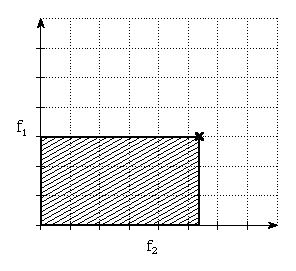
\includegraphics[width=\textwidth]{img/mokp/dom-def}
        \caption{Região de dominância de uma solução.}
        \label{fig:dom-def}
    \end{subfigure}
    \qquad
    \begin{subfigure}[t]{0.3\textwidth}
        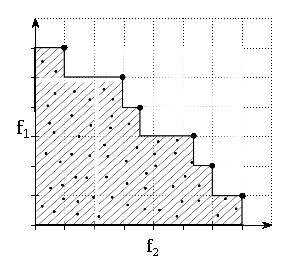
\includegraphics[width=\textwidth]{img/mokp/pareto-def}
        \caption{Exemplo de \paretoset.}
        \label{fig:eff-def}
    \end{subfigure}
    \caption{Exemplos de solução dominante e \paretoset.}
    \label{fig:mo-defs}
\end{figure}

%%% Intro ao MOKP

Um dos problemas multiobjetivos mais importantes da literatura
é o problema da mochila multiobjetivo (\mokp{}).
Muitas problemas reais podem ser modelados como uma instância do \mokp{}
como seleção de projetos~\cite{teng1996multiobjective},
orçamento de capital~\cite{rosenblatt1989generating},
carregamento de carga~\cite{teng1996multiobjective}
e planejamento de estoque~\cite{ishibuchi2015behavior}.

\missing{Comentar sobre a dificuldade de problemas MObj.
Exploão do pareto com o aumento da quantidade de objectivos.
Poucos métodos extados eficientes, geralmente utiliza-se métodos heurísticos.}

%%%%%%%%%%%%%%%%%%%%%%%%%
%%% Definição do MOKP %%%
%%%%%%%%%%%%%%%%%%%%%%%%%
O problema da mochila multi-objetivo pode ser descrito como uma função vetorial
$f$ que mapeia uma variável de decisão (solução) a uma tupla de $\np$ valores
(objetivos).
Formalmente:
\begin{align*}
  \text{max} ~ \sol{y} &= f(\sol{x}) =
    \big(f_1(\sol{x})
    ,f_2(\sol{x})
    ,\ldots
    ,f_{\np}(\sol{x})\big) \\
  \text{sujeito a} ~ \sol{x} & \in X
\end{align*}
onde $\sol{x}$ é a \emph{variável de decisão}, $X$ denota o conjunto de
soluções viáveis e $\sol{y}$ representa o \emph{vetor de objetivos} para os quais
deseja-se maximizar.

Vale resaltar que o tamanho do \paretoset para o problema em questão
tende a crescer rapidamente com o tamanho do problema, especialmente com o
número de objetivos.

Uma instância de um problema da mochila multi-objetivo (\mokp{}) com $\np$
objetivos consiste em uma capacidade inteira $W >0$ e $n$ itens.
Cada item $i$ possui um peso inteiro positivo $w_i$ e $\np$ lucros inteiros
$p_i^1, p_i^2, \ldots, p_{i}^{\np}$ não negativos.
O lucro $p_i^k$ representa a contribuição do $i$-ésimo item
para com o $k$-ésimo objetivo.
Uma solução é representada por um conjunto $\sol{x} \subseteq \{1, \ldots, n\}$
contendo os índices dos itens incluídos na mochila.
Uma solução é viável se o peso total incluído na mochila não ultrapassa
a capacidade da mochila.
Formalmente a definição do problema é a seguinte:
\begin{align*}
  \text{max   } & f(x) =
    \big(f_1(x) ,f_2(x) ,\ldots ,f_{\np}(x)\big) \\
  \text{subject to   } & w(x) \leq W \\
  & x \in \{0, 1\}^n\\
  \text{where} \phantom{mmmmm} \\
  %I_n &= \{1, \ldots, n\}\\
  f_j(x) &= \sum_{i = 1}^n p^j_i x_i \quad j = 1, \ldots, \np\\
  w(x) &= \sum_{i = 1}^n w_i x_i
\end{align*}

O \mokp{} é considerado um problema \nphard{} visto set uma generalização
do bem conhecido problema da mochila $0-1$, para o qual $\np = 1$.
É consideravelmente difícil determinar o \paretoset para um \mokp{},
especialmente para vários objetivos.
Até mesmo para casos bi-objetivos, problemas pequenos podem se apresentar
intratáveis.
Por este motivo interessa-se no desenvolvimento de métodos eficientes
para manipular uma grande quantidade de soluções, o que pode eventualmente
trazer tratabilidade a instâncias antes intratáveis.

A literatura contém várias propostas para resolver o \mokp{} de forma exata.
Porém, nenhum método tem provado ser eficiente para grande instâncias
com mais de dois objetivos.
Mesmo para problemas bi-objetivo, algumas instâncias de tamanho considerado
médio têm aprestando difculdades na determinação da solução exata, o que
tem motivado o desenvolvimento de métodos heurísticas que buscam determinar
um \paretoset aproximado em tempo computacional razoável.


\section{Literature Review}
Several exact approaches have been proposed in the literature for
solving the MOKP.
Examples of such approaches are
the theoretical work
on~\cite{klamroth2000dynamic} where several
dynamic programming formulations are presented,
a $\varepsilon$-constraint method presented in \cite{chankong2008multiobjective},
the two-phase method including a branch and bound algorithm proposed
in~\cite{visee1998two}, a labeling method presented
in~\cite{captivo2003solving} and the dynamic programming
algorithm proposed in~\cite{bazgan2009} which is the most
efficient exact algorithm according to literature.
Some later contributions for the dynamic programming approach
are an algorithmic improvement for bi-objective
cases~\cite{figueira2013algorithmic},
techniques for reducing its memory usage~\cite{correia2018} and
a multi-dimensional solution indexing strategy for performance
improvement~\cite{baroni2017}.

One of the main difficulties on multi-objective optimization problems
is the large cardinality of the set of non-dominated (or \emph{efficient}) solutions,
which has motivated research to provide an approximation of the solution
set~\cite{bazgan2015approximate, vanderpooten2017covers}.
Indeed, it is well-known, in particular, that most multi-objective combinatorial
optimization problems are \emph{intractable}, in the sense that
the number of non-dominated points is exponential in the size of the instance
\cite{ehrgott2013multicriteria}, which motivates the use of heuristics.

Most of proposed multi-objective metaheuristic are adaptations
of metaheuristics originally proposed for single-objective cases.
Among these we may mention
a simulated annealing algorithm~\cite{czyzzak1998pareto},
a scatter search based method~\cite{da2006scatter,da2007integrating},
a tabu search-based method~\cite{gandibleux2000tabu},
%a cooperative swarm intelligence~\cite{zouache2018cooperative},
a quantum inspired artificial immune system~\cite{gao2014quantum},
a hybrid genetic algorithm~\cite{abdelaziz1999hybrid} and
an estimation of distribution method~\cite{martins2017hybrid}.

One of the most popular heuristic algorithm for the MOKP
is the nondominated sorting genetic algorithm (NSGA-II)
proposed in~\cite{deb2002fast}.
This algorithm uses sorts based on the dominance concept
to obtain the convergence towards the Pareto optimal set.
It also employs the crowding distance to maintain the diversity
of the solution set.

Another common heuristic algorithm is the Strength Pareto
Evolutionary Algorithm (SPEA-II), proposed in~\cite{zitzler2001spea2}.
SPEA-II is a genetic algorithm that, in contrast
to NSGA-II, is based on the use of a external population
called archive.
This external population contains a limited number of
non-dominated solutions during the optimization phase.
At any iteration, the new non-dominated solutions of the
population are compared to members of the archive
with respect to dominance.

Recently a cooperative swarm intelligence algorithm called
MOFPA has been proposed in~\cite{zouache2018cooperative},
combing a firefly algorithm and a particle swarm
optimization for cooperation on the exploration of the search space.
A transfer function is used for discretization of the solutions.
The results are compared with NSGA-II, SPEA-II and other 3
algorithms.
The experiments showed that this novel approach 
out-performed the other algorithms in terms of convergence
to optimal while preserving good diversity of solutions.

% Capitulo 3
\chapter{The Multi-dimensional Indexing}
\label{cap:kdtree}
In this chapter we propose the use of a multi-dimensional
indexing structure for handling MOKP solutions.
The strategy is applied as a performance improvement
on a state of art exact algorithm for the MOKP.
Computational experiments verifies the efficiency of the approach.

\section{Dominance Check as Range Search Operation}
\label{sec:kdtree}
% Falar sobre a utilização de estrutura de dados.

\section{Verificação de dominância e a busca de faixa}

Como dito anteriormente, solucionar um problema multi-objetivo significa
apresentar o seu \paretoset{}, ou seja, o conjunto de soluções não dominadas.
Geralmente o processo de solução compreende-se em contruir este conjunto de
soluções de forma incremental.
Por este motivo, um dos procedimentos mais executados durante o processo é
verificar se uma determinada solução é dominada por alguma outra solução
existente num conjunto candidato.
Um algoritmo pode até mesmo necessitar de extrair um cojunto cobertura, ou seja,
extrair todas as soluções não-dominadas de um grande conjuto de soluções.

Esta operação deve demandar exforço quadrático sobre o número total de soluções
se implementada como uma comparação par-a-par.
Entretanto, se as soluções forem interpretadas como pontos em um espaço
multi-dimensional, podemos deduzir da Equação~\ref{eq:dom} que esta operação
corresponde em verificar a existência um ponto numa determinada região
do espaço. O mesmo pode ser considerado no caso mais específico para a dominância
da mochila, segundo a Equação~???.
Formalmente:
\begin{align*}
    & x \dom y \; \Longleftrightarrow \; \pnt{y} \in R(\sol{x}) \\
  \text{where} \phantom{mmmmm} \\
    \pnt{x} &= \big(\obj{1}{x}, \ldots, \obj{\np}{x}, \weight{x}\big) \\
    R(\sol{x}) &= \left\{ a \in \mathbb{R}^{\np+1} \;\middle|\;
      a_{\np+1} \leq \weight{x}
      \, \text{ and } \,
      a_i \geq \obj{i}{x}, \; i \in \{1, \ldots, \np\}
      \right\}
\end{align*}

\missing{Colocar referência para a equação de dominância da mochila (texto acima).}

O problema de determinar a existência de um ponto numa determinada região do
espaço é já bem conhecido da computação e chama-se problema da
\emph{busca de baixa} (ou \emph{range search} em ingês)~\cite{agarwal1999geometric}.
O problema de busca de faixa é largamente aplicado, por exemplo, na área da
computação gráfica e jogos, onde é necessário se verificar a colisão entre pontos e polígonos.
Para se ter uma solução eficiente deste problema evitando o esforço computacional
quadrático, os pontos devem ser indexados multidimensional.....
\missing{Melhorar parágrafo acima e conferir texto inicial do parágrafo abaixo.}

Devido a sua simplicidade e eficiência, a estrutura de dados mais utilizada
para o problema é a \emph{\kdtree}~\cite{preparata2012computational}.
Proposta por Jon Louis Bentley em 1957~\cite{bentley1975}, a \kdtree{} é um tipo de
árvore binária de construção simples e baixa utilização de memória.
Apesar de sua simplicidade, além da operação de buca de faixa, a \kdtree{}
suporta outras operações como busca de vizinho mais próximo.
Por este motivo é também bastante utilizada em algoritmos de
clasterização~\cite{kanungo2002efficient, indyk1998approximate}
e renderização gráfica~\cite{owens2007survey}.

Como uma árvore binária comum, a cada nível recursivo da árvore
a \kdtree{} subdivide os dados em duas partes.
Porém, diferentemente de uma árvore de busca binária comum, as quais utilizam
apenas uma \emph{chave} em todos os níveis da árvore, a \kdtree{} utiliza um
total de $k$ chaves fazendo um revezamento circular entre as chaves à medida
que caminha nos níveis da árvore.

A Figura~\ref{fig:kdom-kd} apresenta (a) um conjunto de pontos dispostos num
espaço bi-dimensional e indexados por uma (b) \dtree{2}.
O primeiro e terceiro nível da \dtree{2} indexa a componente $x$ dos pontos,
enquanto o segundo nível indexa a componente $y$.
Cada ponto indexado pela árvore subdivide o espaço em dois de acordo
com o valor da componente que está sendo indexada.
A subdivisão do espaço é representada na figura por uma linha mais grossa.

\begin{figure}
  \centering
  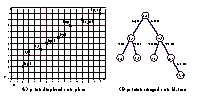
\includegraphics[scale=4.8]{img/kdt/dom-kd}
  \caption{Exemplo de pontos indexados por uma \kdtree{}.}
  \label{fig:kdom-kd}
\end{figure}

A Figura~\ref{fig:query} apresenta um exemplo de operação de verificação de
dominância utilizando uma \dtree{2} como estrutura de indexação.
A área acinzentada não tem intersecção com a área dominada pelo ponto $x$
(área hachurada), portanto as soluções dentro da área acinzentada não são
avaliadas.

\missing{Propor passo-a-passo da operação.}

\begin{figure}
  \centering
  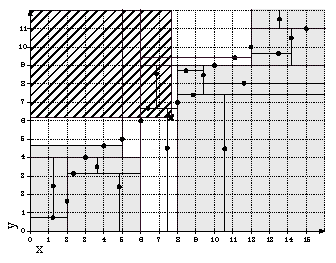
\includegraphics[scale=1.7]{img/kdt/query}
  \caption{Exemplo de operação de verificação de dominância utilizando a \kdtree{}.}
  \label{fig:query}
\end{figure}

Com relação à eficiência da \kdtree{} é importante considerar que não é
recomendável escalar de forma arbitrária o número $k$ de dimensões
indexadas pela \kdtree{}, esperando assim escalar também sua eficiência.
Mesmo que o dado possua todas estas dimensões.
Como regra geral considera-se que um \kdtree{} é adequada para indexar um
conjunto com $n$ pontos se $n$ não for muito maior que $2^k$\cite{toth2004handbook},
caso contrário, a performance da \kdtree{} se assemelhará a de uma busca
linear exaustiva.

Espera-se que a \kdtree{} auxilie as operações de verificação de dominância
\emph{podando} uma grande quantidade de soluções, demandando um menor número
de comparações entre soluções, melhorando assim a performance dos algoritmos.

% Falar um pouco sobre arvore binária.

% Definir a árvore kdtree


\section{The DP Algorithm -- A Use Case}
% Breve resumo sobre métodos de programação dynamica
% Explicação overview do método para o MOKP
% - Process overview of DP for MKP
% - Dom. relations
% - Application of dom. rel.
\cite{bazgan2009}


% Basic simple Dynamic Programming
% Nemhauser-Ullmann algorithm



\subsection{Computational Experiments}
Several computational experiments were performed with the objective of
verifying the efficiency of multi-dimensional indexing on the algorithm,
especially for instances with higher dimensions.
All instances were generated in the same manner as described in~\cite{bazgan2009}.
Four types of bi-objective instances were considered:
\begin{enumerate}
  \item[A)] Random instances: $
    p^j_i \in [1, 1000],
    w_i \in [1,1000]$.
  \item[B)] Unconflicting instances: $
    p^1_i \in [111, 1000],\\
    p^2_i \in [p^1_i - 100, p^1_i + 100],\\
    w_i \in [1,1000]$.
  \item[C)] Conflicting instances: $
    p^1_i \in [1, 1000],\\
    p^2_i \in [max\{900-p^1_i;1\}, min\{1100-p^1_i, 1000\}],\\
    w_i \in [1,1000]$.
  \item[D)] Conflicting instances with correlated weight: $
    p^1_i \in [1, 1000],\\
    p^2_i \in [max\{900-p^1_i;1\}, min\{1100-p^1_i, 1000\}],\\
    w_i \in [p^1_i+p^2_i-200, p^1_i+p^2_i+200]$.
\end{enumerate}
where $\in [a,b]$ denotes uniformly randomly generated in range $[a,b]$.
Instances of type B are considered the easiest ones
while type D are considered the hardest.
For all instances, we set $W=\frac{1}{2}\floor{\sum^n_{k=1} w^k}$.
For each type and each value of $n$ 10 different instances were generated.
The experiments were run on a Intel\textsuperscript{\textregistered}
Core\textsuperscript{TM} i5-3570 3.40HGz computer with 4GB of RAM and
the algorithms were implemented in C programming language.

\begin{table}[]
  \centering
  \begin{tabular}{crr|r|rr}
  \hline
  %%%%%%%%%%%%%%%%%
  %   HEADER
  %%%%%%%%%%%%%%%%%
  \multicolumn{3}{c|}{Instance}
  & AVL tree
  & \multicolumn{2}{c}{\dtree{2}}
    \\
  Type
  & $n$
  & $|ND| $
  & time (s)
  & time (s)
  & speedup
    \\ \hline
\multirow{2}{*}{A}
 &  40 &   38.1 & \textbf{0.06} & \textbf{  0.06} &  1.0 \\
 &  60 &   73.1 &    1.12 & \textbf{  0.88} &  1.3 \\
 &  80 &  125.6 &   19.81 & \textbf{ 11.89} &  1.7 \\
 & 100 &  180.4 &  165.24 & \textbf{ 76.50} &  2.2 \\
 & 120 &  233.9 &  708.53 & \textbf{361.87} &  2.0 \\ \hline
\multirow{2}{*}{B}
 & 100 &    3.1 & \textbf{  0.02} &    0.08 &  0.3 \\
 & 200 &   10.0 & \textbf{  0.80} &    5.09 &  0.2 \\
 & 300 &   24.9 & \textbf{  9.45} &   88.30 &  0.1 \\
 & 400 &   36.2 & \textbf{ 95.39} &  730.04 &  0.1 \\
 & 500 &   53.7 & \textbf{255.57} & 2824.65 &  0.1 \\
 \hline
\multirow{2}{*}{C}
 &  20 &   36.6 & \textbf{0.00} & \textbf{   0.00} &  1.0 \\
 &  40 &  102.8 &    0.65 & \textbf{   0.42} &  1.5 \\
 &  60 &  231.9 &   28.98 & \textbf{  14.09} &  2.1 \\
 &  80 &  358.0 &  564.10 & \textbf{ 241.54} &  2.3 \\
 & 100 &  513.8 & 3756.57 & \textbf{1605.19} &  2.3 \\ \hline
\multirow{2}{*}{D}
 &  20 &  174.9 &    0.15 & \textbf{   0.12} &  1.3 \\
 &  30 &  269.3 &   16.82 & \textbf{   7.60} &  2.2 \\
 &  40 &  478.0 &  395.76 & \textbf{ 186.67} &  2.1 \\
 &  50 &  553.4 & 2459.48 & \textbf{1417.94} &  1.7 \\ \hline
\end{tabular}

  \caption{Average CPU-time for bi-objective instances.}
  \label{tab:cpu2dim}
\end{table}

Table~\ref{tab:cpu2dim} presents results on bi-objective instances
where $|ND|$ is the size of the solution set.
The last column of the table shows the speedup of using \dtree{2}.
Fig.~\ref{fig:cmp2dim} presents the number of solutions
evaluations for bi-objective cases.
The horizontal axis presents the number of items.
Each presented value is the average for 10 instances.

It can be noted that the use of \dtree{2} 
increased the performance of
the algorithm with a speedup up to $2.3$ on instances
of type A, C and D, which have large solution sets.
In most cases occurred the reduction of almost
an order of magnitude in the number of solution evaluations.
For instances of type B the use of \dtree{2} had a poor performance,
even with the reduction in the number of evaluations.
This is probably to the small size of the solution set
for which the use of the structure is not efficient.

\begin{figure}[]
  \centering
\begin{subfigure}{.5\textwidth}
  \centering
  \input{tab/cmp/2dimA.tex}
  \caption{Type A}
  \label{fig:sub1}
\end{subfigure}%
\begin{subfigure}{.5\textwidth}
  \centering
  \input{tab/cmp/2dimB.tex}
  \caption{Type B}
  \label{fig:sub2}
\end{subfigure}
\begin{subfigure}{.5\textwidth}
  \centering
  \input{tab/cmp/2dimC.tex}
  \caption{Type C}
  \label{fig:sub3}
\end{subfigure}%
\begin{subfigure}{.5\textwidth}
  \centering
  \input{tab/cmp/2dimD.tex}
  \caption{Type D}
  \label{fig:sub4}
\end{subfigure}
  \caption{Average number of solution evaluations for bi-objective instances.}
  \label{fig:cmp2dim}
\end{figure}

For the experiments with $3$-objective cases
we considered the generalization introduced in \cite{bazgan2009}
for the bi-dimensional types A and C,
and proposed the generalization of types B and D as follows:
\begin{enumerate}
  \item[A)] Random instances: $
    p^j_i \in [1, 1000]\\
    w_i \in [1,1000]$
  \item[B)] Unconflicting instances: $
    p^1_i \in [111, 1000],\\
    p^2_i \in [p^1_i - 100, p^1_i + 100],\\
    p^3_i \in [p^1_i - 100, p^1_i + 100],\\
    w_i \in [1,1000]$.
  \item[C)] Conflicting instances: $
    p^1_i \in [1, 1000], \;
    p^2_i \in [1, 1001 - p^1_i] \\
    p^3_i \in [max\{900-p^1_i-p^2_i;1\}, min\{1100-p^1_i-p^2_i, 1001-p^1_i\}]\\
    w_i \in [1,1000]$.
  \item[D)] Conflicting instances with correlated weight: $
    p^1_i \in [1, 1000]\\
    p^2_i \in [1, 1001 - p^1_i] \\
    p^3_i \in [max\{900-p^1_i-p^2_i;1\}, min\{1100-p^1_i-p^2_i, 1001-p^1_i\}]\\
    w_i \in [p^1_i+p^2_i+p^3_i-200, p^1_i+p^2_i+p^3_i+200]$.
\end{enumerate}

\begin{table}[]
  \centering
  \begin{tabular}{crr|r|rc|rc}
  \hline
  %%%%%%%%%%%%%%%%%
  %   HEADER
  %%%%%%%%%%%%%%%%%
  \multicolumn{3}{c|}{Instance}
  & AVL tree
  & \multicolumn{2}{c|}{\dtree{2}}
  & \multicolumn{2}{c}{\dtree{3}}
    \\
  Type
  & $n$
  & $|ND| $
  & time (s)
  & time (s)
  & speedup
  & time (s)
  & speedup
    \\ \hline
  %%%%%%%%%%%%%%%%%
  %   CLASS A
  %%%%%%%%%%%%%%%%%
  \multirow{2}{*}{A}
  & 50 &  557.5 &    41.2 &    21.3 & 1.9 & \textbf{  18.5} & 2.2 \\
  & 60 & 1240.0 &   485.9 &   247.8 & 1.9 & \textbf{  79.9} & 6.0 \\
  & 70 & 1879.3 &  3179.5 &  1038.0 & 3.0 & \textbf{ 614.5} & 5.1 \\
  & 80 & 2540.5 &  6667.9 &  3796.0 & 1.7 & \textbf{2943.9} & 2.2 \\
  & 90 & 3528.5 & 24476.5 & 12916.7 & 1.8 & \textbf{3683.7} & 6.6 \\ \hline
  %%%%%%%%%%%%%%%%
  %   CLASS B
  %%%%%%%%%%%%%%%%%
  \multirow{2}{*}{B}
  & 100 &  18.0 & \textbf{   0.1} &    0.3 & 0.3 &    0.3 & 0.3 \\
  & 200 &  65.4 & \textbf{  11.4} &   34.4 & 0.3 &   29.1 & 0.4 \\
  & 300 & 214.2 & \textbf{ 307.7} &  631.5 & 0.5 &  583.2 & 0.5 \\
  & 400 & 317.0 & \textbf{4492.9} & 8464.9 & 0.5 & 5402.2 & 0.8 \\ \hline
  %%%%%%%%%%%%%%%%%
  %   CLASS C
  %%%%%%%%%%%%%%%%%
  \multirow{2}{*}{C}
  & 20 &  254.4 &   0.06 &   0.05 & 1.2 & \textbf{ 0.03} & 2.17 \\
  & 30 & 1066.6 &   9.69 &   4.18 & 2.3 & \textbf{ 1.30} & 7.46 \\
  & 40 & 2965.5 & 471.68 & 153.21 & 3.1 & \textbf{30.50} & 15.5 \\ \hline
  %%%%%%%%%%%%%%%%
  %   CLASS D
  %%%%%%%%%%%%%%%%%
  \multirow{2}{*}{D}
  & 20 & 4087.7 &   23.6 &   10.9 & 2.2 & \textbf{   1.9} & 12.5 \\
  & 30 & 8834.5 & 8914.2 & 3625.3 & 2.5 & \textbf{1019.5} &  8.7 \\ \hline
\end{tabular}
  \caption{Average CPU-time for 3-objective instances.}
  \label{tab:cpu3dim}
\end{table}

\begin{figure}[]
  \centering
\begin{subfigure}{.5\textwidth}
  \centering
  %\input{tab/cmp/3dimA.tex}
  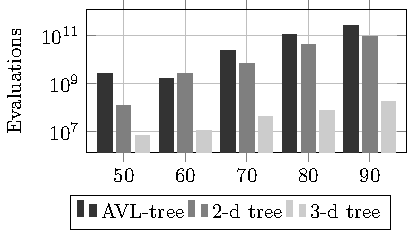
\includegraphics[scale=1.1]{tab/cmp/3dimA}
  \caption{Tipo A}
  \label{fig:sub5}
\end{subfigure}%
\begin{subfigure}{.5\textwidth}
  \centering
  %\input{tab/cmp/3dimB.tex}
  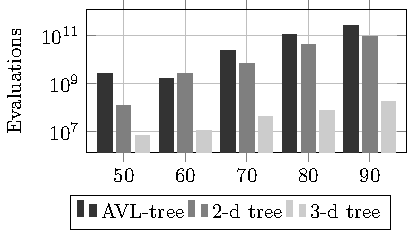
\includegraphics[scale=1.1]{tab/cmp/3dimA}
  \caption{Tipo B}
  \label{fig:sub6}
\end{subfigure}
\begin{subfigure}{.49\textwidth}
  \centering
  %\input{tab/cmp/3dimC.tex}
  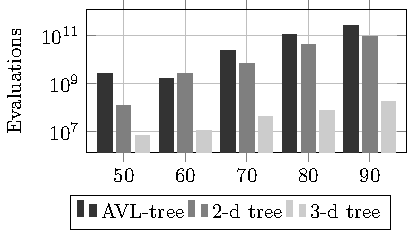
\includegraphics[scale=1.1]{tab/cmp/3dimA}
  \caption{Tipo C}
  \label{fig:sub7}
\end{subfigure}
\begin{subfigure}{.49\textwidth}
  \centering
  %\input{tab/cmp/3dimD.tex}
  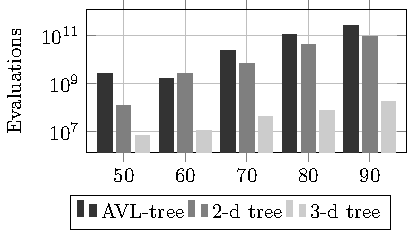
\includegraphics[scale=1.1]{tab/cmp/3dimA}
  \caption{Tipo D}
  \label{fig:sub8}
\end{subfigure}

  \caption{Average number of solution evaluations for 3-objective instances.}
  \label{fig:cmp3dim}
\end{figure}

Table~\ref{tab:cpu3dim} shows results on 3-objective instances for which
were used AVL tree, \dtree{2} and \dtree{3}.
Fig.~\ref{fig:cmp3dim} presents the number of solutions evaluations for 3-objective cases.
Each presented value is the average for 10 instances.

The use of multi-dimensional indexing for all 3-objective cases
increased the performance of the algorithm with \dtree{3}
outperforming \dtree{2} on types A, C and D.
The use of \kdtree{} still had lower performance on type B.


\subsection{Conclusions}
This chapter shows the application of a multi-dimensional indexing structure
for exactly solving the MOKP with a dynamic programming algorithm
and investigating its efficiency.
Through computational experiments we showed that multi-dimensional indexing
is applicable to the problem requiring considerably less solution evaluations,
especially on hard instances,
which resulted in a algorithm speedup $2.3$ for bi-dimensional
cases and up to $15.5$ on 3-dimensional cases.
The multi-dimensional indexing was not efficient on \emph{easy} instances
for which the set of solutions is relatively small.

Despite the considerable performance improvement
provided by the multi-dimensional indexing strategy,
several instances are still intractable due 
the large number of intermediate solutions,
especially for 3-objective cases.
For this reason this work proposes to use the indexing strategy
in conjunction with an evolutionary metaheuristic
which is expected to provide
promising results for hard instances,
particularly for many-objective instances.

The following chapter will introduce the shuffled complex algorithm
and presents is application for efficiently solves
the multi-dimensional knapsack problem.
\label{sec:dynprogcomp}

% Capitulo 4
\chapter{The Shuffled Complex Evolution}
\label{cap:sce}
The SCE is a population
based evolutionary optimization algorithm 
proposed by Duan in \cite{duan1992effective}
and has been successfully used on scheduling problems~\cite{zhao2015shuffled},
project management~\cite{elbeltagi2007modified},
$0-1$ knapsack problems~\cite{bhattacharjee2014shuffled} and
multi-dimensional knapsack problem~\cite{baroni2015shuffled,baroni2016shuffled}.
This chapter introduces the SCE algorithm presenting its
application for solving the multi-dimensional knapsack problem
with the assistance of a variable fixing procedure specific for the problem.

\section{Definition}
\label{sec:sce}

%
\begin{frame}
\frametitle{}
\begin{center}
  \textbf{\Large The Shuffled Complex Evolution}
\end{center}
\end{frame}

%
\begin{frame}
\frametitle{The Shuffled Complex Evolution}
\begin{columns}
\begin{column}{0.75\textwidth}  %%<--- here
  {\small
  The SCE  regards a natural  evolution happening
  simultaneously in independent communities;
  \\ \medskip \pause
  A population of $N*M$ individuals is randomly taken from the
  solution space;
  \\ \medskip \pause
  The population is then sorted by descending order of fitness
  and the best global solution is identified;
  \\ \medskip \pause
  The population is then shuffled into $N$ complexes,
  each containing $M$ individuals;
  \\ \medskip \pause
  In this shuffling process the first individual goes to the first complex, the second
  individual goes to the second complex, individual $N$ goes to $N$-th complex,
  individual $(M+1)$-th goes back to the first complex, etc;
  \\ \medskip \pause
  The next step after shuffling the complexes is to evolve each complex.
  }
\end{column} \pause
\begin{column}{0.25\textwidth}
  \hspace{-15pt}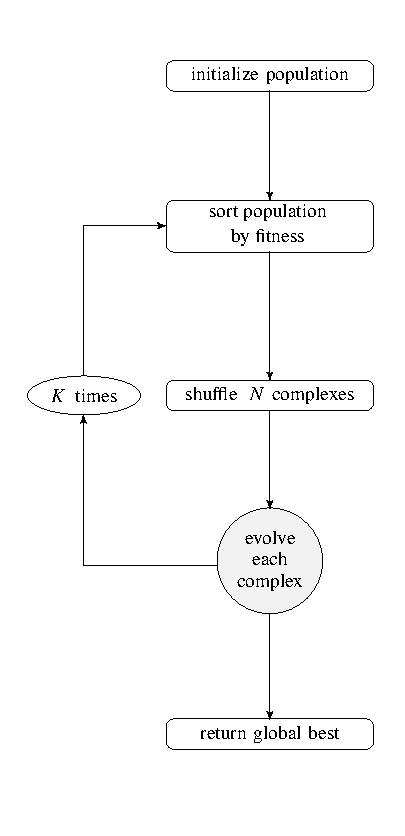
\includegraphics[scale=0.45]{img/sce/flow1}
\end{column}
\end{columns}
\end{frame}

%
\begin{frame}
\frametitle{The Shuffled Complex Evolution}
\begin{columns}
\begin{column}{0.75\textwidth}  %%<--- here
  {\small
  In each step a subcomplex of $P$ individuals is selected from the
  complex;
  \\ \medskip \pause
  After the selection of the subcomplex, its worst individual is identified to
  be replaced by a new generated solution;
  \\ \medskip \pause
  This new solution is generated by the crossing of the worst individual and an
  other individual with better fitness;
  \\ \medskip \pause
  At first the best individual of the subcomplex is considered for the crossing;
  \\ \medskip \pause
  If the new solution is not better than the worst one, the best individual
  of the complex is considered for a crossing;
  \\ \medskip \pause
  If the latter crossing did not result in any improvement, the best individual
  of whole population is considered;
  \\ \medskip \pause
  Finally, if all the crossing steps couldn't generate a better individual,
  the worst individual of the subcomplex is replaced by a new random solution taken
  from the feasible solution space.
  }
\end{column} \pause
\begin{column}{0.25\textwidth}
  \vspace{10pt}\hspace{-18pt}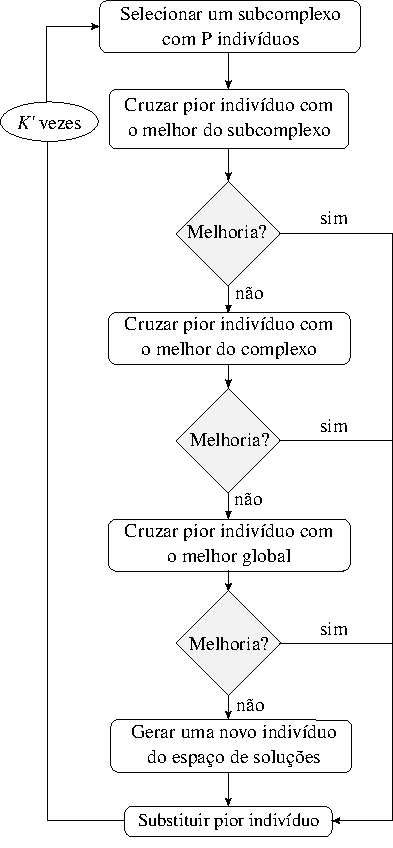
\includegraphics[scale=0.45]{img/sce/flow2}
\end{column}
\end{columns}
\end{frame}

%
\begin{frame}
\frametitle{}
\begin{center}
  \textbf{\Large The Shuffled Complex Evolution}
  \\ \bigskip \bigskip
  {\large Use case for the MKP}
\end{center}
\end{frame}

% The SCE for MKP
\begin{frame}
\frametitle{The SCE for MKP}
the SCE is easily applied to any
optimization problem.
The only steps needed to be specified is \textbf{(a)} the creation of a new random
solution and \textbf{(b)} the crossing procedure of two solutions.
\end{frame}

% Random for MKP
\begin{frame}
\frametitle{The SCE for MKP}
New random solution generation for the MKP.
\begin{figure}
\begin{algorithmic}[1]
  \Function{New random solution}{} \pause
    \State $v \leftarrow $ shuffle($1, 2, \ldots, n$) \pause
	\State $s \leftarrow \emptyset$ \pause
    \For{$ i \leftarrow 1:n$ }
	  \State $s \leftarrow s \cup \{v_i\}$ \pause
	  \If{ $s$ is not feasible} \pause
	    \State $s \leftarrow s - \{v_i\}$
      \EndIf  \pause
	\EndFor
  \State return $s$
  \EndFunction
\end{algorithmic}
\end{figure}
\end{frame}

% Crossing for MKP
\begin{frame}
\frametitle{The SCE for MKP}
Crossing procedure for the MKP.
\begin{figure}
\begin{algorithmic}[1]
  \Function{Crossing}{$x^w:$ worst individual, $x^b:$ better individual, $c$} \pause
    \State $v \leftarrow $ shuffle($1, 2, \ldots, n$) \pause
    \For{$ i \leftarrow 1:c$ }
	  \State $j \leftarrow v_i$ \pause
	  \State $x^w_j \leftarrow x^b_j$
	\EndFor \pause
	\If{$s^w$ is not feasible}
	  \State repair $s^w$
	\EndIf \pause
  \State return $s^w$
  \EndFunction
\end{algorithmic}
\end{figure}
\end{frame}


% SCE parameters
\begin{frame}
\frametitle{Computational Experiments}
Parameters used for SCE:
\begin{itemize}
  \item $N = 20$: number of complexes;
  \item $M = 20$: number of individuals in each complex;
  \item $P = 5$: number of individuals in each subcomplex;
  \item $K = 300$: number of algorithm iterations;
  \item $K' = 20$: number of iterations used in the complex evolving process;
  \item $c = n/5$: number of genes carried from parent in crossing process.
\end{itemize}
\end{frame}

% Results (chub)
\begin{frame}
\frametitle{Computational Experiments}
SCE and \scecore  performance on Chu-Beasley problems.
\begin{table}[hb]
{
\renewcommand{\arraystretch}{0.7}%
\fontsize{4.5pt}{1em}\selectfont
\begin{center}
  \begin{tabular}{rrr|cc|cc} \hline
  \multirow{2}{*}{\bf n} &
  \multirow{2}{*}{\bf m} &
  \multirow{2}{*}{\textbf{$\alpha$}} &
    \multicolumn{2}{c|}{\textbf{time} (s)} &
    \multicolumn{2}{c}{\textbf{quality}(\%)} \\
  &
    &
    &
    \textbf{SCE} &
    \textbf{\scecore} &
    \textbf{SCE} &
    {\bf \scecore}  \\ \hline
100   &  5 & 0.25 & 1.22\fvar{0.04} & \textbf{0.17}\fvar{0.00} & 96.51\fvar{0.92} & \textbf{99.73}\fvar{0.04} \\
        &    & 0.50 & 1.34\fvar{0.02} & \textbf{0.18}\fvar{0.00} & 97.42\fvar{0.55} & \textbf{99.86}\fvar{0.01} \\
        &    & 0.75 & 1.37\fvar{0.03} & \textbf{0.17}\fvar{0.00} & 98.87\fvar{0.20} & \textbf{99.91}\fvar{0.00} \\ \cline{2-7}
        & 10 & 0.25 & 1.32\fvar{0.04} & \textbf{0.25}\fvar{0.00} & 95.68\fvar{1.28} & \textbf{99.53}\fvar{0.09} \\
        &    & 0.50 & 1.51\fvar{0.04} & \textbf{0.25}\fvar{0.00} & 96.65\fvar{0.49} & \textbf{99.76}\fvar{0.03} \\
        &    & 0.75 & 1.46\fvar{0.04} & \textbf{0.27}\fvar{0.00} & 98.54\fvar{0.19} & \textbf{99.96}\fvar{0.00} \\ \cline{2-7}
        & 30 & 0.25 & 1.74\fvar{0.06} & \textbf{1.20}\fvar{0.03} & 95.38\fvar{1.01} & \textbf{97.96}\fvar{0.22} \\
        &    & 0.50 & 1.79\fvar{0.08} & \textbf{0.89}\fvar{0.06} & 96.41\fvar{0.63} & \textbf{99.18}\fvar{0.06} \\
        &    & 0.75 & 1.72\fvar{0.09} & \textbf{0.95}\fvar{0.04} & 98.18\fvar{0.33} & \textbf{99.52}\fvar{0.04} \\ \hline
\multirow{2}{*}{250} & 5 & 0.25 & 2.87\fvar{0.07} & \textbf{0.69}\fvar{0.01} & 93.22\fvar{0.64} & \textbf{99.86}\fvar{0.00} \\
        &    & 0.50 & 2.82\fvar{0.11} & \textbf{0.70}\fvar{0.01} & 94.88\fvar{0.21} & \textbf{99.94}\fvar{0.00} \\
        &    & 0.75 & 2.93\fvar{0.08} & \textbf{0.69}\fvar{0.01} & 97.57\fvar{0.10} & \textbf{99.96}\fvar{0.00} \\ \cline{2-7}
        & 10 & 0.25 & 3.08\fvar{0.09} & \textbf{0.87}\fvar{0.01} & 93.14\fvar{0.67} & \textbf{99.58}\fvar{0.01} \\
        &    & 0.50 & 3.03\fvar{0.09} & \textbf{0.79}\fvar{0.02} & 94.55\fvar{0.26} & \textbf{99.79}\fvar{0.00} \\
        &    & 0.75 & 3.12\fvar{0.09} & \textbf{0.84}\fvar{0.01} & 97.16\fvar{0.13} & \textbf{99.88}\fvar{0.00} \\ \cline{2-7}
        & 30 & 0.25 & 3.74\fvar{0.12} & \textbf{1.52}\fvar{0.04} & 93.10\fvar{0.74} & \textbf{98.42}\fvar{0.08} \\
        &    & 0.50 & 3.74\fvar{0.16} & \textbf{1.36}\fvar{0.06} & 94.20\fvar{0.30} & \textbf{99.33}\fvar{0.02} \\
        &    & 0.75 & 3.99\fvar{0.13} & \textbf{1.48}\fvar{0.04} & 96.64\fvar{0.14} & \textbf{99.59}\fvar{0.01} \\ \hline
\multirow{2}{*}{500} & 5 & 0.25 & 5.62\fvar{0.10} & \textbf{1.25}\fvar{0.02} & 91.37\fvar{0.50} & \textbf{99.77}\fvar{0.00} \\
        &    & 0.50 & 5.72\fvar{0.19} & \textbf{1.24}\fvar{0.01} & 93.39\fvar{0.27} & \textbf{99.88}\fvar{0.00} \\
        &    & 0.75 & 5.88\fvar{0.14} & \textbf{1.20}\fvar{0.02} & 96.42\fvar{0.06} & \textbf{99.92}\fvar{0.00} \\ \cline{2-7}
        & 10 & 0.25 & 5.97\fvar{0.17} & \textbf{1.41}\fvar{0.02} & 91.62\fvar{0.50} & \textbf{99.51}\fvar{0.01} \\
        &    & 0.50 & 6.11\fvar{0.23} & \textbf{1.36}\fvar{0.03} & 93.09\fvar{0.20} & \textbf{99.77}\fvar{0.00} \\
        &    & 0.75 & 5.47\fvar{0.61} & \textbf{1.21}\fvar{0.03} & 96.24\fvar{0.06} & \textbf{99.84}\fvar{0.00} \\ \cline{2-7}
        & 30 & 0.25 & 6.20\fvar{1.14} & \textbf{1.96}\fvar{0.22} & 91.37\fvar{0.82} & \textbf{98.76}\fvar{0.02} \\
        &    & 0.50 & 6.26\fvar{1.07} & \textbf{1.82}\fvar{0.14} & 92.56\fvar{0.13} & \textbf{99.42}\fvar{0.01} \\
        &    & 0.75 & 6.05\fvar{1.16} & \textbf{1.73}\fvar{0.20} & 95.97\fvar{0.06} & \textbf{99.67}\fvar{0.00} \\ \hline
\end{tabular}

\end{center}
}
\end{table}
\end{frame}

% Results (gk)
\begin{frame}
\frametitle{Computational Experiments}
\scecore performance on Glover-Kochenberger problems.
\begin{table}[hb]
  {
  \renewcommand{\arraystretch}{1}%
  \fontsize{5.5pt}{1em}\selectfont
  \begin{center}
    \begin{tabular}{rrr|cc|rr} \hline
  \multirow{2}{*}{\textbf{\#}} &
  \multirow{2}{*}{\textbf{n}} &
  \multirow{2}{*}{\textbf{m}} &
    \multicolumn{2}{c|}{\textbf{time}(s)} &
    \multicolumn{2}{c}{\textbf{quality}(\%)} \\
  &
    &
    &
    \textbf{SCE} &
    \textbf{SCEcr} &
    \textbf{SCE} &
    \textbf{SCEcr} \\ \hline
  01   &  100 &  15 &   1.47\fvar{0.00} & \textbf{0.08}\fvar{0.0} & 97.66\fvar{0.03} & \textbf{99.24}\fvar{0.02} \\ \hline
    02 &  100 &  25 &   1.61\fvar{0.00} & \textbf{0.09}\fvar{0.0} & 97.94\fvar{0.04} & \textbf{98.94}\fvar{0.09} \\ \hline
    03 &  150 &  25 &   2.51\fvar{0.01} & \textbf{0.09}\fvar{0.0} & 97.22\fvar{0.04} & \textbf{99.09}\fvar{0.02} \\ \hline
    04 &  150 &  50 &   3.56\fvar{0.03} & \textbf{0.09}\fvar{0.0} & 97.40\fvar{0.04} & \textbf{98.52}\fvar{0.02} \\ \hline
    05 &  200 &  25 &   3.55\fvar{0.01} & \textbf{0.09}\fvar{0.0} & 96.88\fvar{0.03} & \textbf{99.28}\fvar{0.01} \\ \hline
    06 &  200 &  50 &   4.81\fvar{0.09} & \textbf{0.10}\fvar{0.0} & 97.68\fvar{0.02} & \textbf{98.90}\fvar{0.03} \\ \hline
    07 &  500 &  25 &   7.30\fvar{0.09} & \textbf{0.10}\fvar{0.0} & 97.12\fvar{0.01} & \textbf{99.54}\fvar{0.00} \\ \hline
    08 &  500 &  50 &  12.20\fvar{0.47} & \textbf{0.11}\fvar{0.0} & 97.27\fvar{0.01} & \textbf{99.33}\fvar{0.01} \\ \hline
    09 & 1500 &  25 &  24.61\fvar{1.73} & \textbf{0.12}\fvar{0.0} & 95.40\fvar{0.01} & \textbf{98.22}\fvar{0.00} \\ \hline
    10 & 1500 &  50 &  33.79\fvar{2.44} & \textbf{0.13}\fvar{0.0} & 97.50\fvar{0.00} & \textbf{99.64}\fvar{0.00} \\ \hline
    11 & 2500 & 100 & 121.28\fvar{194.74} & \textbf{0.15}\fvar{0.0} & 97.95\fvar{0.00} & \textbf{99.70}\fvar{0.00} \\ \hline
\end{tabular}

  \end{center}
  }
\end{table}
\end{frame}

% Results (gk)
\begin{frame}
\frametitle{Conclusions}
The SCE algorithm for MKP proved to be able to achieve fast
convergence ratio, finding good quality near optimal solutions, demanding small
amount of computational time.
\\ \medskip \pause
The core concept as a variable fixing procedure
proved to be efficient to reduce the size of the problems which provided fast
execution time, producing higher quality solutions.
\\ \medskip \pause
At least $99.02\%$ of best known, in less than $2$ seconds for every instance.
\end{frame}


\section{A SCE for the MKP}
\label{sec:scemkp}
The multi-dimensional knapsack problem (MKP) is a strongly NP-hard combinatorial
optimization problem which can be viewed as a resource allocation problem and
defined as follows:
\begin{align}
  \text{maximize} & \sum_{j=1}^n p_j x_j \\
  \text{subject to} & \sum_{j=1}^n w_{ij} x_j \leqslant c_i \quad i \in \{1, \ldots, m\}\\
   & x_j \in \{0, 1\}, \quad j \in \{1, \ldots, n\}.
\end{align}

% Define the MKP
The problem can be interpreted as a set of $n$ items with profits $p_j$
and a set of $m$ resources with capacities $c_i$.
Each item $j$ consumes an amount $w_{ij}$ from each resource $i$, if selected.
The objective is to select a subset of items with maximum total profit,
not exceeding the defined resource capacities.
The decision variable $x_j$ indicates if $j$-th item is selected.
It is considered an integer programming problem (IP) since its variables $x_i$
are restricted to be integers.

The multi-dimensional knapsack problem can be applied on budget planning 
scenarios and project selections~\cite{mcmillan1973resource},
cutting stock problems~\cite{Gilmore-Gomory-1966}, loading problems~\cite{Shih-1979},
allocation of processors and databases in distributed computer programs~\cite{Gavish-Pirckul-1982}.

The problem is a generalization of the well-known knapsack problem (KP) in which
$m = 1$.
However it is a NP-hard problem significantly harder to solve in practice than the KP.
%Despite the existence of a fully polynomial approximation scheme (FPAS) for the KP,
%finding a FPAS for the MKP is NP-hard for $m \geqslant 2$~\cite{magazine1984note}.
Due its simple definition but challenging difficulty of solving, the MKP is often used to
to verify the efficiency of novel metaheuristics.

Its well known that the hardness of a NP-hard problem grows exponentially over
its size.
Thereupon, a suitable approach for tackling NP-hard problems is to reduce their size
through some variable fixing procedure.
Despite not guaranteeing optimality of the solution, an efficient variable
fixing procedure may provide near optimal solutions through a small computational effort.

%A metaheuristic is a set of concepts that can be used to define heuristic methods
%that can be applied to a wide set of different problems.
%In other words, a metaheuristic can be seen as a general algorithmic framework which can be applied to
%different optimization problems with relatively few modifications to make them adapted to a specific problem.”
As it can be noted in its description the SCE is easily applied to any
optimization problem.
The only steps needed to be specified is (a) the creation of a new random
solution and (b) the crossing procedure of two solutions.
The procedures presented in this section are based
on the work in \cite{baroni2015shuffled}.
These two procedures for the MKP are respectively presented by algorithms on
Figure~\ref{alg:new} and Figure~\ref{alg:cross}.

To construct a new random solution (Figure~\ref{alg:new}) the items are
at first shuffled in random order and stored in a list (line 2).
A new empty solution is then defined (line 3).
The algorithm iteratively tries to fill the solution's knapsack with 
the an item taken from the list (lines 4-9).
The feasibility of the solution is then checked: if the item insertion let
the solution unfeasible (line 6) its removed from knapsack (line 7).
After trying to place all available items the new solution is returned.

\begin{figure}
\begin{algorithmic}[1]
  \Procedure{Crossing}{$x^w:$ worst individual, $x^b:$ better individual, $c$}
    \State $v \leftarrow $ shuffle($1, 2, \ldots, n$)
    \For{$ i \leftarrow 1:c$ }
	  \State $j \leftarrow v_i$
	  \State $x^w_j \leftarrow x^b_j$ \Comment{gene carriage}
	\EndFor
	\If{$s^w$ is not feasible}
	  \State repair $s^w$
	\EndIf
	\State update $s^w$ fitness
  \State return $s^w$
  \EndProcedure
\end{algorithmic}
\caption{Crossing procedure used on SCE algorithm.}
\label{alg:cross}
\end{figure}

The crossing procedure (Figure~\ref{alg:cross}) takes as input the worst
solution taken from the subcomplex $x^w = (x^w_1, x^w_2, \ldots, x^w_n$),
the selected better solution $x_b = (x^b_1, x^b_2, \ldots, x^b_n$)
and the number $c$ of genes that will be carried from the better solution.
The $c$ parameter will control how similar the worst individual will be from the
given better individual.
At first the items are shuffled in random order and stored in a list (line 2).
Then $c$ randomly chosen genes are carried from the better individual to the worst
individual (line 5).
At the end of steps the feasibility of the solution is checked (line 7) and
the solution is repaired if needed.
The repair stage is a greedy procedure that iteratively removes the item that less
decreases the objective function.
Finally the fitness of the generated solution is updated (line 10) and
returned (line 11).

The following section will present the core concept for the MKP.
The concept will be used as a problem reduction
technique that will assist the SCE method as a pre-processing
step on the algorithm.
Its application on the SCE algorithm for the MKP is
also a contribution of this work.

\subsection{The Core Concept for the MKP}
\label{sec:core}

The core concept was first presented for the one-dimensional 0-1 knapsack problem (KP),
leading to very successful KP algorithms.
The main idea is to reduce the original problem by only considering a set of
items for which it is hard to decide if they will occur or not in an optimal solution.
This set of items is named core.
The variables for all items outside the core are fixed to certain values.

The knapsack problem considers items $j = 1, \ldots, n$, associated profits $p_j$ and
associated weights $w_j$.
A subset of these items has to be selected and packed into a knapsack having capacity $c$.
The total profit of the items in the knapsack has to be maximized, while the
total weight is not allowed to exceed $c$.

Before defining the core of the KP it is worth to note the solution structure
of its LP-relaxation.
The LP-relaxation of an integer programming problem arises by replacing the
constraint that each variable must be integer by a constraint that allows
continuity of the variable.
The LP-relaxation of a KP is found by replacing the constraint $x_i \in \{0,1\}$
by $0 \leqslant x_i \leqslant 1$ for all $i \in \{1, \ldots, n\}$.
If the items are sorted according to decreasing efficiency values
\begin{equation}
  e_j = \frac{p_j}{w_j},
\end{equation}
it is known that the solution of the LP-relaxation consists of
three consecutive parts: the first part contains variables set to $1$, the second
pare consists of at most one split item $s$, whose corresponding LP-values is
fractional, and finally the remaining variables, which are always set to zero,
form the third part.

For most instance of KP (except those with a very special structure) the integer
optimal solution closely corresponds to this partitioning in the sense that it
contains most of the highly efficient items of the first part, some items with
medium efficiency near the split item, and almost no items with low efficiency
from the third part.
Items of medium efficiency constitute the core.

Balas and Zemel~\cite{balas1980algorithm} gave the following precise definition
of the core of a KP, based on the knowledge of an optimal integer solution $x^*$.
Assume that the items are sorted according to decreasing efficiency and let
\begin{equation}
  a := \min\{ j | x_j^* = 0 |\}, \quad b := \max\{ j | x_j^* = 1 \}.
\end{equation}
The core is given by the items in the interval $C = \{a, \ldots, b\}$.
It is obvious that the split item is always part of the core, i.e., $a < s < b$.

Figure~\ref{fig:kpecore} illustrates an exact core for an hypothetical KP instance
with $13$ items.
First row represents the efficiency value $e$ of each item.
The items are sorted by descending order of efficiency.
Second row represent solution array of the LP-relaxation.
The third row represents the exact solution for the original problem.
The $8$-th item is the split item.
Notice that the split item is within the exact core.

\begin{figure}[ht]
  \centering
  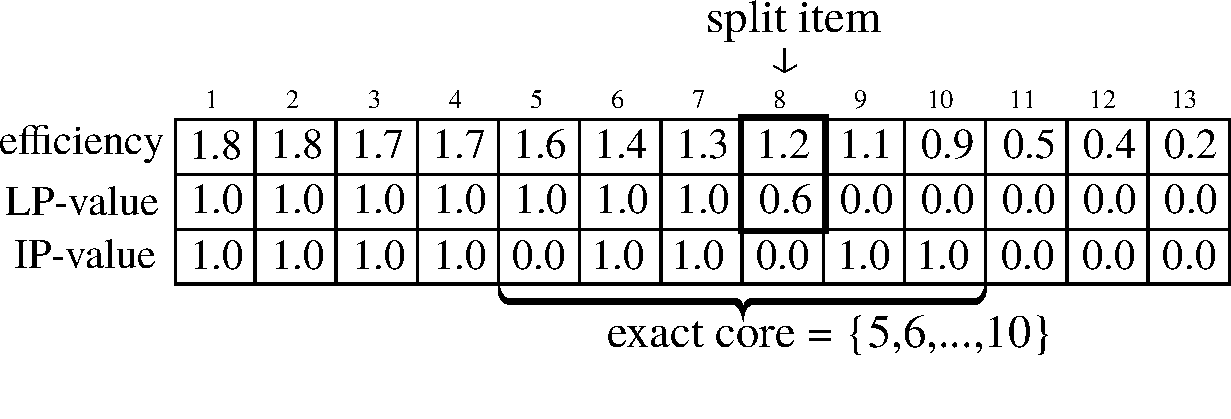
\includegraphics[scale=0.406]{img/sce/core}
  \caption{Example of exact core for a hypothetical KP instance.}
  \label{fig:kpecore}
\end{figure}

The KP Core problem (KPC) is defined as
\begin{align}
  \text{maximize} & \sum_{j \in C} p_j x_j  + \tilde{p}\\
  \text{subject to} & \sum_{j \in C} w_{j} x_j \leqslant c - \tilde{w}\\
  & x_j \in \{0, 1\}, \quad j \in C.
\end{align}
with $\tilde{p} = \sum^{a-1}_{j=1} p_j$ and $\tilde{w} = \sum^{a-1}_{j=1} w_j$
respectively quantifying the total profit and the total weights of items fixed as selected.
The solution of KPC would suffice to compute the optimal solution of KP, which
however, has to be already partially known to determine $C$.
Nevertheless an approximate core $C = \{s-\delta, \ldots, s+\delta\}$,
of fixed size $|C| = 2\delta+1$ is considered for a heuristic reduction of the problem.

Figure~\ref{fig:kpcore} exemplifies an approximate core of a hypothetical KP
instance with $13$ items.
The first row represents the efficiency value of each item and the second row
represents the value of each variable on the LP-relaxation optimal solution.
The items are sorted in descending order of efficiency value.
The last row illustrates the variable fixing after the defined core.
Asterisks indicate free variables associated to the items in the
approximate core.

\begin{figure}[ht]
  \centering
  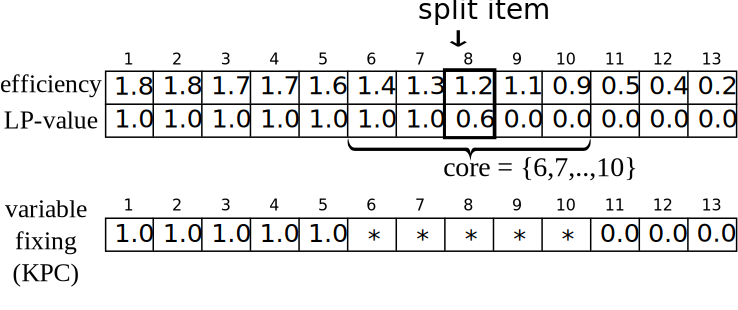
\includegraphics[scale=0.406]{img/sce/kp_3}
  \caption{Example of core for a hypothetical KP instance with $n=13$ and approximate core size of $5$ ($\delta = 2$).}
  \label{fig:kpcore}
\end{figure}

%\subsubsection{The Core Concept for MKP}

The previous definition of the core for KP can be extended to MKP without major
difficulties, once an efficiency measure is defined for the MKP,
as addressed in \cite{puchinger2006core}, even though,
a proper efficiency measure for MKP is not obvious due the
multidimensional weight of the items.
A well accepted efficiency measure is discussed in Section~\ref{subsec:dual}.

Now let $x^*$ be an optimal solution for a MKP and assume that the items are
sorted in descending order after some given efficiency measure. Then let
\begin{align}
  a = \min \{ j | x_j^* = 0 \}, \quad b = \max \{ j | x_j^* = 1 \}.
\end{align}
The core is given by the items in the interval $C = \{ a, \ldots, b \}$,
and the multidimensional knapsack core problem (MKPC) defined as
\begin{align}
  \text{maximize} & \sum_{j \in C} p_j x_j  + \tilde{p}\\
  \text{subject to} & \sum_{j \in C} w_{ij} x_j \leqslant c_i - \tilde{w}_i, \quad i = 1, \ldots, m\\
  & x_j \in \{0, 1\}, \quad j \in C.
\end{align}
with $\tilde{p} = \sum^{a-1}_{j=1} p_j$  and $\tilde{w}_i = \sum^{a-1}_{j=1} w_{ij}, i = 1, \ldots, m$.

In contrast to KP, the solution of the LP-relaxation of MKP in general does not
consists of a single fractional split item. But up to $m$ fractional values give
rise to a whole \emph{split interval} $S = \{ s_1, \ldots, s_m\}$, where
$s_1$ and $s_m$ are respectively the first and the last index of variables with
fractional values after sorting by the given efficiency measure.
Once the split interval is defined, a central index value $s = \lfloor \frac{s_1+s_m}{2}\rfloor$
can be used as the center of an approximate core.

%\subsubsection{The Dual-variable Efficiency Measure}
\label{subsec:dual}
For defining a reasonable efficiency measure for MKP consider the most obvious
form of efficiency which is a direct generalization of the one-dimensional case:
\begin{equation}
	e_j(simple) = \frac{p_j}{\sum_{i=1}^{m} w_{ij}}
\end{equation}
In this definition different orders of magnitude of the constraints are not
considered and a single constraint may dominate the others.
This drawback can be avoided by introducing relevance values $r_i$ for every
constraint:
\begin{equation}
	e_j(relevance) = \frac{p_j}{\sum_{i=1}^{m} r_i w_{ij}}
\end{equation}
Several proposals for setting the relevance values $r_i$ were discussed and
tested by Puchinger, Raidl and Pferschy in \cite{puchinger2006core}.
According to their work setting the relevance values $r_i$ to the values of an
optimal solution to the dual problem of the MKP's LP-relaxation, as suggested
in \cite{Chu-Beasley-1998}, achieved the best results and will be the one
considered in this work for the development of the hybrid heuristic.

While the original MKP can be seen as a resource allocation problem,
the dual problem of the MKP can be seen as a resource valuation problem.
For this reason the values of the dual solution is related to the
\emph{importance} of each resource.

The split interval resulting from the efficient measure considered can be
precisely characterized.
Let $x^{LP}$ be the optimal solution of the LP-relaxation of MKP.
Then the following relation holds, as proved in \cite{puchinger2006core}:
\begin{displaymath}
 x_l^{LP} =
  \begin{cases}
    1         & \mbox{if } e_j > 1, \\
    \in [0,1] & \mbox{if } e_j = 1, \\
    0         & \mbox{if } e_j < 1.
  \end{cases}
\end{displaymath}
From this relation we can note that all variables in the split interval will
have efficiency measure $e_j = 1$, while less and more efficient ones will have
$e_j < 1$ and $e_j > 1$ respectively.

Figure~\ref{fig:mkpcore} exemplifies an approximate core of a hypothetical MKP
with $13$ variables and $3$ dimensions.
Notice that the LP-relaxation solution has now $3$ fractional variables that
defines the center of the split interval.

\begin{figure}[ht]
  \centering
  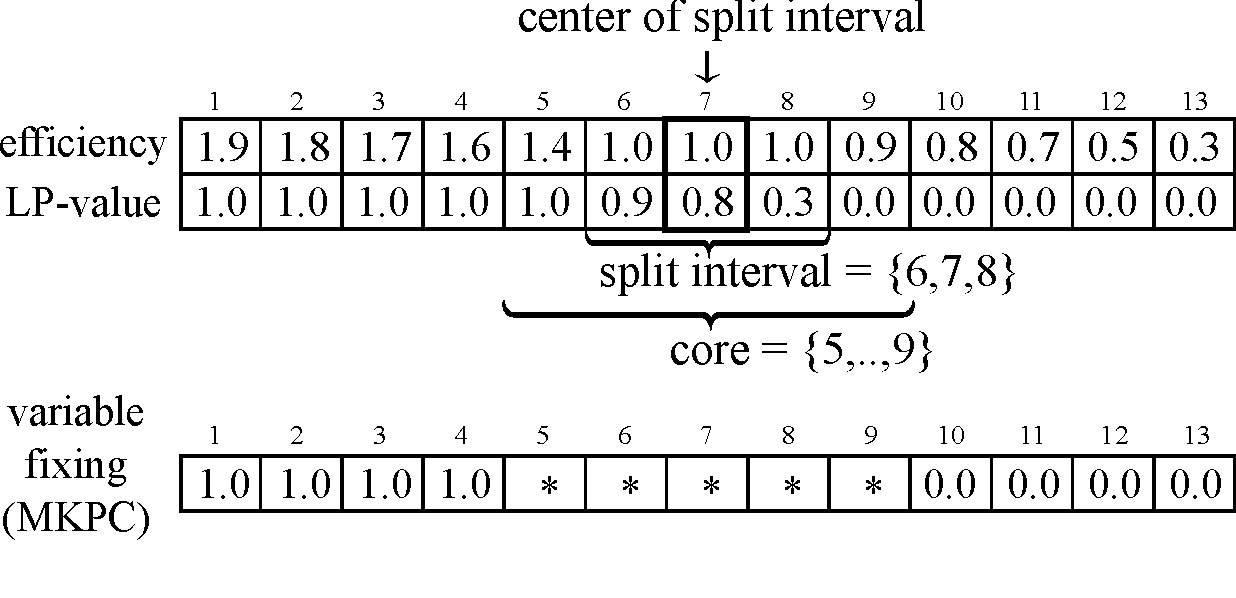
\includegraphics[scale=0.406]{img/sce/mkp_3}
  \caption{Example of core for a hypothetical MKP instance with $n=13$, $m=3$ and approximate core size of $5$ ($\delta = 2$).}
  \label{fig:mkpcore}
\end{figure}

The core will be applied as a problem reduction procedure
for fixing a given number of variables of the problem,
before being inputted to the SCE algorithm.
The following section presents computational experiments for
evaluating the approach.


\subsection{Computational Experiments}
\label{sec:scemkpcomp}
To verify the efficiency of the proposed metaheuristic, several computational
experiments was executed considering the original SCE for the MKP
without using the problem reduction procedure -- as proposed in \cite{baroni2015shuffled} --
and the SCE with the reduction procedure.
For brevity the SCE with the reduction procedure will be referred to as \scecore.

For the experiments, two sets of MKP instances was used:
a first set composed by 270 instances provided by Chu and Beasley (\cite{Chu-Beasley-1998})
and a second set composed by 11 instances provided by Glover and Kochenberger in
\cite{glover1996critical}.
These instances are all available at \cite{ORLibrary}.

The best known solution for all instances were taken from the literature and
were found by different algorithms which we had no access to the implementation.
In mosts cases those are exact algorithms which took
minutes or hours of execution time.

The set of MKP instances provided by Chu and Beasley was generated using a
procedure suggested by Freville and Plateau~\cite{freville1994efficient}, which
attempts to generate instances hard to solve.
The number of constraints $m$ varies among $5$, $10$ and $30$, and the number
of variables $n$ varies among $100$, $250$ and $500$.

The $w_{ij}$ were integer numbers drawn from the discrete uniform distribution
$U(0, 1000)$.
The capacity coefficient $c_i$ were set using
$b_i = \alpha\sum_{j=1}^{n} w_{ij}$ where $\alpha$ is a tightness ratio and
varies among $0.25$, $0.5$ and $0.75$.
For each combination of $(m,n,\alpha)$ parameters, $10$ random problems was generated,
totaling $270$ problems.
The profit $p_j$ of the items were correlated to $w_{ij}$ and generated as follows:
\begin{equation}
  p_j = \sum_{i=1}^m \frac{w_{ij}}{m} + 500q_j \qquad j = 1, \ldots, n
\end{equation}

%\subsection{Experimental Results}

All the experiments were run on a Intel$^R$ Core i5-3570 CPU @3.40GHz computer
with 4GB of RAM.
The original SCE and \scecore was both implemented in C programming language.
%For the set of random instance all best known solution was found by the solver
%SCIP 3.0.1 running for at least 10 minutes.

For the variable fixing procedure used on \scecore, the range size of the approximate core was
$|C| = m+\frac{n}{10}$ for all instances.
In all instances the parameters used for SCE and \scecore were the same recommended
in \cite{baroni2015shuffled} which was found after a batch test using Chu and Beasley instances:
\begin{itemize}
  \item $N = 20$: number of complexes;
  \item $M = 20$: number of individuals in each complex;
  \item $P = 5$: number of individuals in each subcomplex;
  \item $K = 300$: number of algorithm iterations;
  \item $K' = 20$: number of iterations used in the complex evolving process;
  \item $c = n/5$: number of genes carried from parent in crossing process.
\end{itemize}

Table~\ref{tab:chu} shows the performance of the SCE and \scecore on the Chu-Beasley set of instances.
Each instance in the set was executed 10 times for each algorithm.
Columns \textit{n}, \textit{m} and \textit{$\alpha$} shows the parameters used
on each instance generation.
The \textit{time} column shows the average execution time of the algorithms (lower is better).
The \textit{quality} column shows the average ratio of the solution found and
the best known solution from literature (\cite{vimont2008reduced, della2012improved}) of each instance (higher is better).
Best values are in bold.

It can be observed that the \scecore had faster convergence speed, achieving higher
quality solutions in all cases, achieving at least $97.96\%$ of best known, in less than $2$ seconds
for every instance.

It can be also noticed that \scecore executed in much less processing time than original
SCE.
This is due the variable fixing procedure which reduced the problem size,
resulting in less genes operations during the evolving procedures.
The variable fixing procedure also brought robustness for the method, as the quality
of the solution found increased in case of larger instances while on original
SCE the quality decreased considerably.

Table~\ref{tab:gk} shows the performance of SCE and \scecore on the Glover-Kochenberger set of instances.
Each instance in the set was executed 10 times for each algorithm.
Columns \textit{n} and \textit{m} indicate the size of each instance.
The \textit{time} column shows the average execution (lower is better).
The \textit{quality} column shows the average ratio of the solution found and
the best known solution of each instance.
Best values are in bold.
It can be noticed that SCEcr achieved high quality solutions, at least $98.22\%$
of best known solution, spending small amount of processing time, compared
to the time taken to find the best known solutions.

\begin{table}[hb]
{
\renewcommand{\arraystretch}{1}%
\fontsize{10.5pt}{1em}\selectfont 
\begin{center}
  \begin{tabular}{rrr|cc|cc} \hline
  \multirow{2}{*}{\bf n} &
  \multirow{2}{*}{\bf m} &
  \multirow{2}{*}{\textbf{$\alpha$}} &
    \multicolumn{2}{c|}{\textbf{time} (s)} &
    \multicolumn{2}{c}{\textbf{quality}(\%)} \\
  &
    &
    &
    \textbf{SCE} &
    \textbf{\scecore} &
    \textbf{SCE} &
    {\bf \scecore}  \\ \hline
100   &  5 & 0.25 & 1.22\fvar{0.04} & \textbf{0.17}\fvar{0.00} & 96.51\fvar{0.92} & \textbf{99.73}\fvar{0.04} \\
        &    & 0.50 & 1.34\fvar{0.02} & \textbf{0.18}\fvar{0.00} & 97.42\fvar{0.55} & \textbf{99.86}\fvar{0.01} \\
        &    & 0.75 & 1.37\fvar{0.03} & \textbf{0.17}\fvar{0.00} & 98.87\fvar{0.20} & \textbf{99.91}\fvar{0.00} \\ \cline{2-7}
        & 10 & 0.25 & 1.32\fvar{0.04} & \textbf{0.25}\fvar{0.00} & 95.68\fvar{1.28} & \textbf{99.53}\fvar{0.09} \\
        &    & 0.50 & 1.51\fvar{0.04} & \textbf{0.25}\fvar{0.00} & 96.65\fvar{0.49} & \textbf{99.76}\fvar{0.03} \\
        &    & 0.75 & 1.46\fvar{0.04} & \textbf{0.27}\fvar{0.00} & 98.54\fvar{0.19} & \textbf{99.96}\fvar{0.00} \\ \cline{2-7}
        & 30 & 0.25 & 1.74\fvar{0.06} & \textbf{1.20}\fvar{0.03} & 95.38\fvar{1.01} & \textbf{97.96}\fvar{0.22} \\
        &    & 0.50 & 1.79\fvar{0.08} & \textbf{0.89}\fvar{0.06} & 96.41\fvar{0.63} & \textbf{99.18}\fvar{0.06} \\
        &    & 0.75 & 1.72\fvar{0.09} & \textbf{0.95}\fvar{0.04} & 98.18\fvar{0.33} & \textbf{99.52}\fvar{0.04} \\ \hline
\multirow{2}{*}{250} & 5 & 0.25 & 2.87\fvar{0.07} & \textbf{0.69}\fvar{0.01} & 93.22\fvar{0.64} & \textbf{99.86}\fvar{0.00} \\
        &    & 0.50 & 2.82\fvar{0.11} & \textbf{0.70}\fvar{0.01} & 94.88\fvar{0.21} & \textbf{99.94}\fvar{0.00} \\
        &    & 0.75 & 2.93\fvar{0.08} & \textbf{0.69}\fvar{0.01} & 97.57\fvar{0.10} & \textbf{99.96}\fvar{0.00} \\ \cline{2-7}
        & 10 & 0.25 & 3.08\fvar{0.09} & \textbf{0.87}\fvar{0.01} & 93.14\fvar{0.67} & \textbf{99.58}\fvar{0.01} \\
        &    & 0.50 & 3.03\fvar{0.09} & \textbf{0.79}\fvar{0.02} & 94.55\fvar{0.26} & \textbf{99.79}\fvar{0.00} \\
        &    & 0.75 & 3.12\fvar{0.09} & \textbf{0.84}\fvar{0.01} & 97.16\fvar{0.13} & \textbf{99.88}\fvar{0.00} \\ \cline{2-7}
        & 30 & 0.25 & 3.74\fvar{0.12} & \textbf{1.52}\fvar{0.04} & 93.10\fvar{0.74} & \textbf{98.42}\fvar{0.08} \\
        &    & 0.50 & 3.74\fvar{0.16} & \textbf{1.36}\fvar{0.06} & 94.20\fvar{0.30} & \textbf{99.33}\fvar{0.02} \\
        &    & 0.75 & 3.99\fvar{0.13} & \textbf{1.48}\fvar{0.04} & 96.64\fvar{0.14} & \textbf{99.59}\fvar{0.01} \\ \hline
\multirow{2}{*}{500} & 5 & 0.25 & 5.62\fvar{0.10} & \textbf{1.25}\fvar{0.02} & 91.37\fvar{0.50} & \textbf{99.77}\fvar{0.00} \\
        &    & 0.50 & 5.72\fvar{0.19} & \textbf{1.24}\fvar{0.01} & 93.39\fvar{0.27} & \textbf{99.88}\fvar{0.00} \\
        &    & 0.75 & 5.88\fvar{0.14} & \textbf{1.20}\fvar{0.02} & 96.42\fvar{0.06} & \textbf{99.92}\fvar{0.00} \\ \cline{2-7}
        & 10 & 0.25 & 5.97\fvar{0.17} & \textbf{1.41}\fvar{0.02} & 91.62\fvar{0.50} & \textbf{99.51}\fvar{0.01} \\
        &    & 0.50 & 6.11\fvar{0.23} & \textbf{1.36}\fvar{0.03} & 93.09\fvar{0.20} & \textbf{99.77}\fvar{0.00} \\
        &    & 0.75 & 5.47\fvar{0.61} & \textbf{1.21}\fvar{0.03} & 96.24\fvar{0.06} & \textbf{99.84}\fvar{0.00} \\ \cline{2-7}
        & 30 & 0.25 & 6.20\fvar{1.14} & \textbf{1.96}\fvar{0.22} & 91.37\fvar{0.82} & \textbf{98.76}\fvar{0.02} \\
        &    & 0.50 & 6.26\fvar{1.07} & \textbf{1.82}\fvar{0.14} & 92.56\fvar{0.13} & \textbf{99.42}\fvar{0.01} \\
        &    & 0.75 & 6.05\fvar{1.16} & \textbf{1.73}\fvar{0.20} & 95.97\fvar{0.06} & \textbf{99.67}\fvar{0.00} \\ \hline
\end{tabular}

\end{center}
}
 \caption{SCE and \scecore  performance on Chu-Beasley problems.}
 \label{tab:chu}
\end{table}

\begin{table}[hb]
{
\renewcommand{\arraystretch}{1}%
\fontsize{10.5pt}{1em}\selectfont 
\begin{center}
  \begin{tabular}{rrr|cc|rr} \hline
  \multirow{2}{*}{\textbf{\#}} &
  \multirow{2}{*}{\textbf{n}} &
  \multirow{2}{*}{\textbf{m}} &
    \multicolumn{2}{c|}{\textbf{time}(s)} &
    \multicolumn{2}{c}{\textbf{quality}(\%)} \\
  &
    &
    &
    \textbf{SCE} &
    \textbf{SCEcr} &
    \textbf{SCE} &
    \textbf{SCEcr} \\ \hline
  01   &  100 &  15 &   1.47\fvar{0.00} & \textbf{0.08}\fvar{0.0} & 97.66\fvar{0.03} & \textbf{99.24}\fvar{0.02} \\ \hline
    02 &  100 &  25 &   1.61\fvar{0.00} & \textbf{0.09}\fvar{0.0} & 97.94\fvar{0.04} & \textbf{98.94}\fvar{0.09} \\ \hline
    03 &  150 &  25 &   2.51\fvar{0.01} & \textbf{0.09}\fvar{0.0} & 97.22\fvar{0.04} & \textbf{99.09}\fvar{0.02} \\ \hline
    04 &  150 &  50 &   3.56\fvar{0.03} & \textbf{0.09}\fvar{0.0} & 97.40\fvar{0.04} & \textbf{98.52}\fvar{0.02} \\ \hline
    05 &  200 &  25 &   3.55\fvar{0.01} & \textbf{0.09}\fvar{0.0} & 96.88\fvar{0.03} & \textbf{99.28}\fvar{0.01} \\ \hline
    06 &  200 &  50 &   4.81\fvar{0.09} & \textbf{0.10}\fvar{0.0} & 97.68\fvar{0.02} & \textbf{98.90}\fvar{0.03} \\ \hline
    07 &  500 &  25 &   7.30\fvar{0.09} & \textbf{0.10}\fvar{0.0} & 97.12\fvar{0.01} & \textbf{99.54}\fvar{0.00} \\ \hline
    08 &  500 &  50 &  12.20\fvar{0.47} & \textbf{0.11}\fvar{0.0} & 97.27\fvar{0.01} & \textbf{99.33}\fvar{0.01} \\ \hline
    09 & 1500 &  25 &  24.61\fvar{1.73} & \textbf{0.12}\fvar{0.0} & 95.40\fvar{0.01} & \textbf{98.22}\fvar{0.00} \\ \hline
    10 & 1500 &  50 &  33.79\fvar{2.44} & \textbf{0.13}\fvar{0.0} & 97.50\fvar{0.00} & \textbf{99.64}\fvar{0.00} \\ \hline
    11 & 2500 & 100 & 121.28\fvar{194.74} & \textbf{0.15}\fvar{0.0} & 97.95\fvar{0.00} & \textbf{99.70}\fvar{0.00} \\ \hline
\end{tabular}

\end{center}
}
 \caption{\scecore performance on Glover-Kochenberger problems.}
 \label{tab:gk}
\end{table}

\subsection{Conclusions}
\label{sec:scemkpconc}
The SCE algorithm, which combines the ideas of a controlled random search with
the concepts of competitive evolution, proved to be able to achieve fast
convergence ratio, finding good quality near optimal solutions, demanding small
amount of computational time.

The application of the core concept as a variable fixing procedure for MKP
proved to be efficient to reduce the size of the problems which provided fast
execution time, producing higher quality solutions.

\scecore algorithm presented faster convergence speed, achieving higher
quality solutions in all cases, achieving at least $99.02\%$ of best known, in less than $2$ seconds
for every instance.
The variable fixing procedure also brought robustness for the method, as the quality
of the solution found increased in case of larger instances.

The heuristic presented in this chapter is very well suitable if it is necessary
to compute a good solution in a small processing time.
The heuristic could achieve $99.61\%$ on average of quality of the best known solution for
the 270 Chu-Beasley instances and $99.46\%$ on average for the Glover-Kochenberger instances.



% Capitulo 5
\chapter{A SCE for the MOKP}
\label{cap:scemokp}
As exposed in previous chapters,
exact methods have difficulties solving several MOKP instances,
especially with more than 2 objectives.
This motivates the development of heuristic methods.
This chapter will discuss the development of
the proposed heuristic algorithm, how tests will be
conducted and analyzed.
A final schedule is presented in the last section.

\section{Algorithm Proposal}
For designing a multi-objective heuristic, one still take into account
two important criteria: (a) how to allow the diversity of solutions
and (b) how to ensure the convergence towards the Pareto optimal set.
The SCE algorithm (a) allows diversity of solutions by evolving independent
sets of solutions which are constructed by shuffling the 
population and (b) ensures convergence by prioritizing
the crossing of individuals with better fitness, which
indicates the potential to compute a good approximate Pareto optimal set.

As seen in previous sections
the SCE is easily applied to any optimization problem.
The fact that the MKP shares the same solution representation
as the MOKP
-- set of items included in the knapsack --
allow us to use the same procedures
presented in Section~\ref{sec:scemkp}
for (a) creating a new random solution
and (b) crossing two solutions.

A crucial point for the successful application of a metaheuristic
on a multi-objective problem is the definition of the fitness function.
One of the most popular multi-objective heuristic algorithms successfully uses sorts
based on the dominance relation for measuring the quality of a solution.
The method is called \emph{non-dominated sort}~\cite{deb2002fast}:
given a set $Q$ of solution, it first selects those which are not dominated
by any other solution in $Q$ to compose the set $S_1$, denoted as
\emph{first non-dominated front}.
Now, all select solutions are removed from $Q$ set and the process
is repeated to make set $S_2$.
The process continues until all fronts are identified.
Solutions in the first fronts are considered the ones with the best fitness.
For tie breaking the aggregation method can be used, which consist of using
a weight vector to compute a scalar over the multiple objective values
of a solution.

A performance issue on the non-dominated sort procedure is
checking if a solutions is dominated by another.
Our propose is to minimize this issue with the assistance
of the indexing strategy proposed in Chapter~\ref{cap:kdtree}.

\section{Computational Experiments and Analyzes}
The proposed algorithm will be tested on the same types
of instances presented  in Chapter~\ref{sec:dynprogcomp},
this time considering 2, 3 and 4 objective cases
and compared with the results that will be obtained from
the MOFPA proposed in~\cite{zouache2018cooperative}.

Two performance metrics will be used to evaluate the
approximation quality of the generated solutions:
(a) set coverage metric~\cite{zitzler1998multiobjective}
and (b) spacing metric~\cite{schott1995fault}:
\begin{itemize}
  \item[(a)]{Set coverage metric ($SC$):
  This metric is intended to be used for comparing
    two non-dominated Pareto sets.
    It defines a semi-distance between two solutions set $A$ and $B$ by:
    \begin{displaymath}
      SC(A, B) = \frac{\big|\{ b \in B
        \;|\; \exists a \in A : dom(a, b)\}\big|}{|B|}
    \end{displaymath}
    This quantity corresponds to the proportion of the solutions
    of the set $B$, that are dominated by at least one solution
    of $A$. It should be noted that $C(A,B)$ is not necessarily
    equal to $1-C(B, A)$. To compare $A$ and $B$ sets, both values
    of  $C(A,B)$ and $C(B,A)$ must be calculated.}
  \item[(b)]{Spacing metric ($SP$): This metric evaluates the uniformity
    of the distribution of non-dominated solutions:
    \begin{displaymath}
      SP(A) = \sqrt{\frac{1}{n-1} \sum^n_{i=1} (\bar{d}-d_i)^2}
    \end{displaymath}
    where $d_i$ is defined as:
    \begin{displaymath}
     d_i = min \sum^M_{m=1} | f^i_m - f^k_m | \qquad k \in A, k \neq i
    \end{displaymath}
    and $\bar{d}$ denotes the average of the distances $d_i$ for
    $i = 1, \ldots, n$.
    $SP$ represents the standard deviation of distance values between
    two consecutive solutions of the set $A$.
    The smaller $SP$, the better distribution of the solutions.
    Moreover, a null value of SP indicates that the solutions are
    equidistant. }
\end{itemize}

The computational results will be reported on a paper to be submitted
to IEEE Congress on Evolutionary Computation 2018 (CEC 2018) that
will be held on July 80-14 in Rio de Janeiro, Brazil.
Its paper submission deadline is January 15.

\newpage
\section{Final Doctoral Schedule}
Table~\ref{tab:sched} presents the final doctoral schedule.

\begin{table}[hb]
\centering
\bgroup
\def\arraystretch{1.1}%
\begin{tabular}{|l|c:c:c|c:c:c:c|c:c:c:c|}
 \hline
  \multirow{3}{*}{\textbf{ \phantom{aaaa} Activities}}
  & \multicolumn{11}{c|}{\textbf{Weeks}} \\ \cline{2-12}
   & \multicolumn{3}{c|}{\textbf{ November }}
   & \multicolumn{4}{c|}{\textbf{December}}
   & \multicolumn{4}{c|}{\textbf{January}} \\ \cline{2-12}
  & \;2º\; & 3º & 4º & 1º & 2º & 3º & 4º & 1º & 2º & 3º & 4º \\ \hline
 Literature review
  & $\bbt$ & $\bbt$ & $\bbt$ & & & & & & & & \\ \hline
 Implementation and adjustments
  & $\bbt$ & $\bbt$ & $\bbt$ & $\bbt$ & & & & & & & \\ \hline
 Computational experiments
  & & & $\bbt$ & $\bbt$ & $\bbt$ & & & & & & \\ \hline
 CEC Paper writing
  & & & & & & $\bbt$ & $\bbt$ & $\bbt$ & & & \\ \hline
 CEC Paper submission
  & & & & & & & & & $\bbt$ & & \\ \hline
 Thesis writing
  & & & & $\bbt$ & $\bbt$ & $\bbt$ & $\bbt$ & $\bbt$ & $\bbt$ & $\bbt$ & \\ \hline
\end{tabular}
\egroup
\caption{Final doctoral schedule.}
\label{tab:sched}
\end{table}

%\vspace{15pt}
%\emph{Métricas de avaliação de solucao, instancias de testes e analises.}


%%%%%%%%%%%%%%%%%%%%%%%%
%  Pós-texto           %
%%%%%%%%%%%%%%%%%%%%%%%%
% ELEMENTOS PÓS-TEXTUAIS
\postextual

% Referências bibliográficas
\bibliography{references}

\end{document}
